% ============================================================
% Figure Captions: Categorical Compound Database
% ============================================================

\begin{figure*}[!htbp]
    \centering
    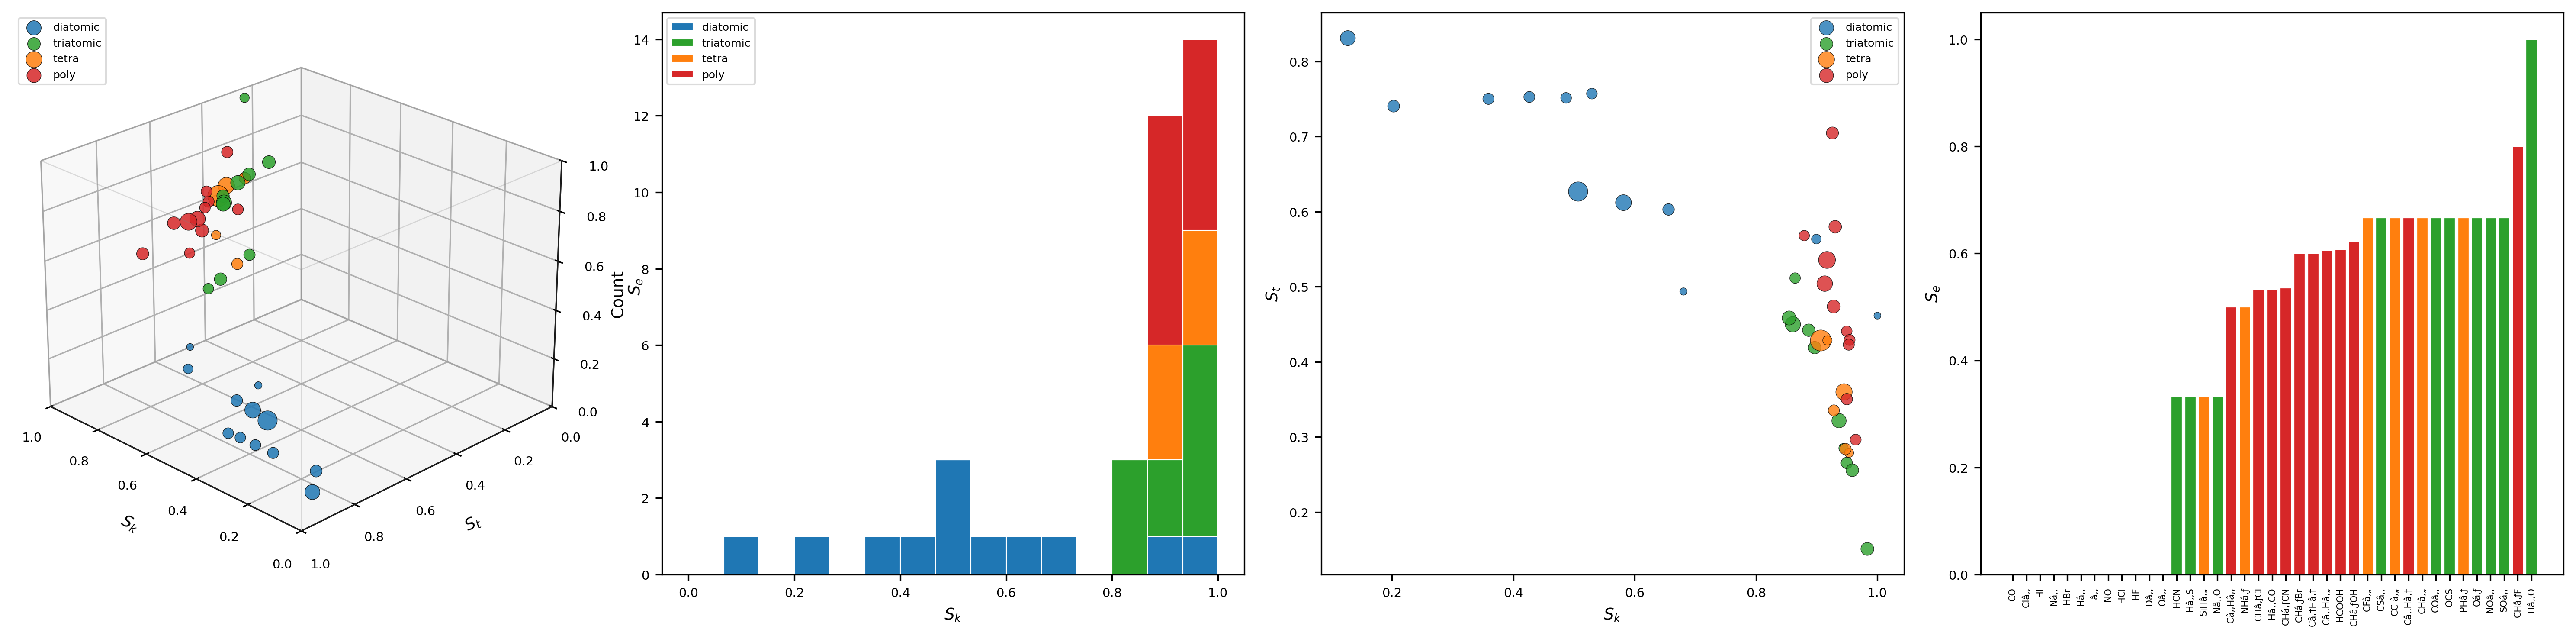
\includegraphics[width=\textwidth]{figures/panel_1_sentropy_space.png}
    \caption{\textbf{S-Entropy Compound Space.}
    (\textbf{A})~All 39 NIST compounds embedded in three-dimensional S-entropy space $\mathcal{S} = [0,1]^3$ with axes $\Sk$ (knowledge entropy), $\St$ (temporal entropy), $\Se$ (evolution entropy). The unit cube wireframe bounds the space. Point size scales with molecular mass; colour encodes molecular type: diatomic (blue), triatomic (green), tetrahedral (orange), polyatomic (red). Diatomics cluster along the $\Se = 0$ plane (no mode pairs, hence no harmonic edges), while polyatomics occupy the interior with $\Se > 0.3$. The clear separation along $\Se$ demonstrates that harmonic network density is the primary discriminant between molecular complexity classes.
    (\textbf{B})~Distribution of knowledge entropy $\Sk$ across the 39 compounds, displayed as stacked histograms coloured by molecular type. Diatomics (blue) span the full $[0.13, 1.00]$ range because their single-mode frequency varies widely ($\mathrm{Cl}_2$ at 560~cm$^{-1}$ to $\mathrm{H}_2$ at 4401~cm$^{-1}$). Polyatomics (red, orange) concentrate near $\Sk \approx 0.9$--$1.0$, reflecting the high Shannon entropy of multi-mode frequency distributions approaching uniformity.
    (\textbf{C})~Temporal entropy $\St$ versus knowledge entropy $\Sk$ for all compounds. Point size scales with molecular mass; colour encodes type. Diatomics occupy the upper-left quadrant (moderate-to-high $\St$, variable $\Sk$), reflecting their large vibrational-to-rotational frequency ratios. Polyatomics cluster in the lower-right quadrant (high $\Sk$, moderate $\St$), where frequency distributions are uniform but the ratio between highest and lowest modes is moderate. The anti-correlation between $\Sk$ and $\St$ for diatomics arises because light diatomics (high $\omega$, high $\Sk$) tend to have moderate rotational constants (moderate $\St$).
    (\textbf{D})~Evolution entropy $\Se$ for all 39 compounds, sorted in decreasing order. Bar colour encodes molecular type. The distribution is clearly bimodal: diatomics at $\Se = 0$ (leftmost bars) and polyatomics/triatomics at $\Se \geq 0.33$. $\mathrm{H}_2\mathrm{O}$ achieves the maximum $\Se = 1.0$ (all three mode pairs are harmonically proximate). The gap between 0 and 0.33 reflects the structural transition from single-mode to multi-mode molecules.}
    \label{fig:sentropy_space}
\end{figure*}

\begin{figure*}[!htbp]
    \centering
    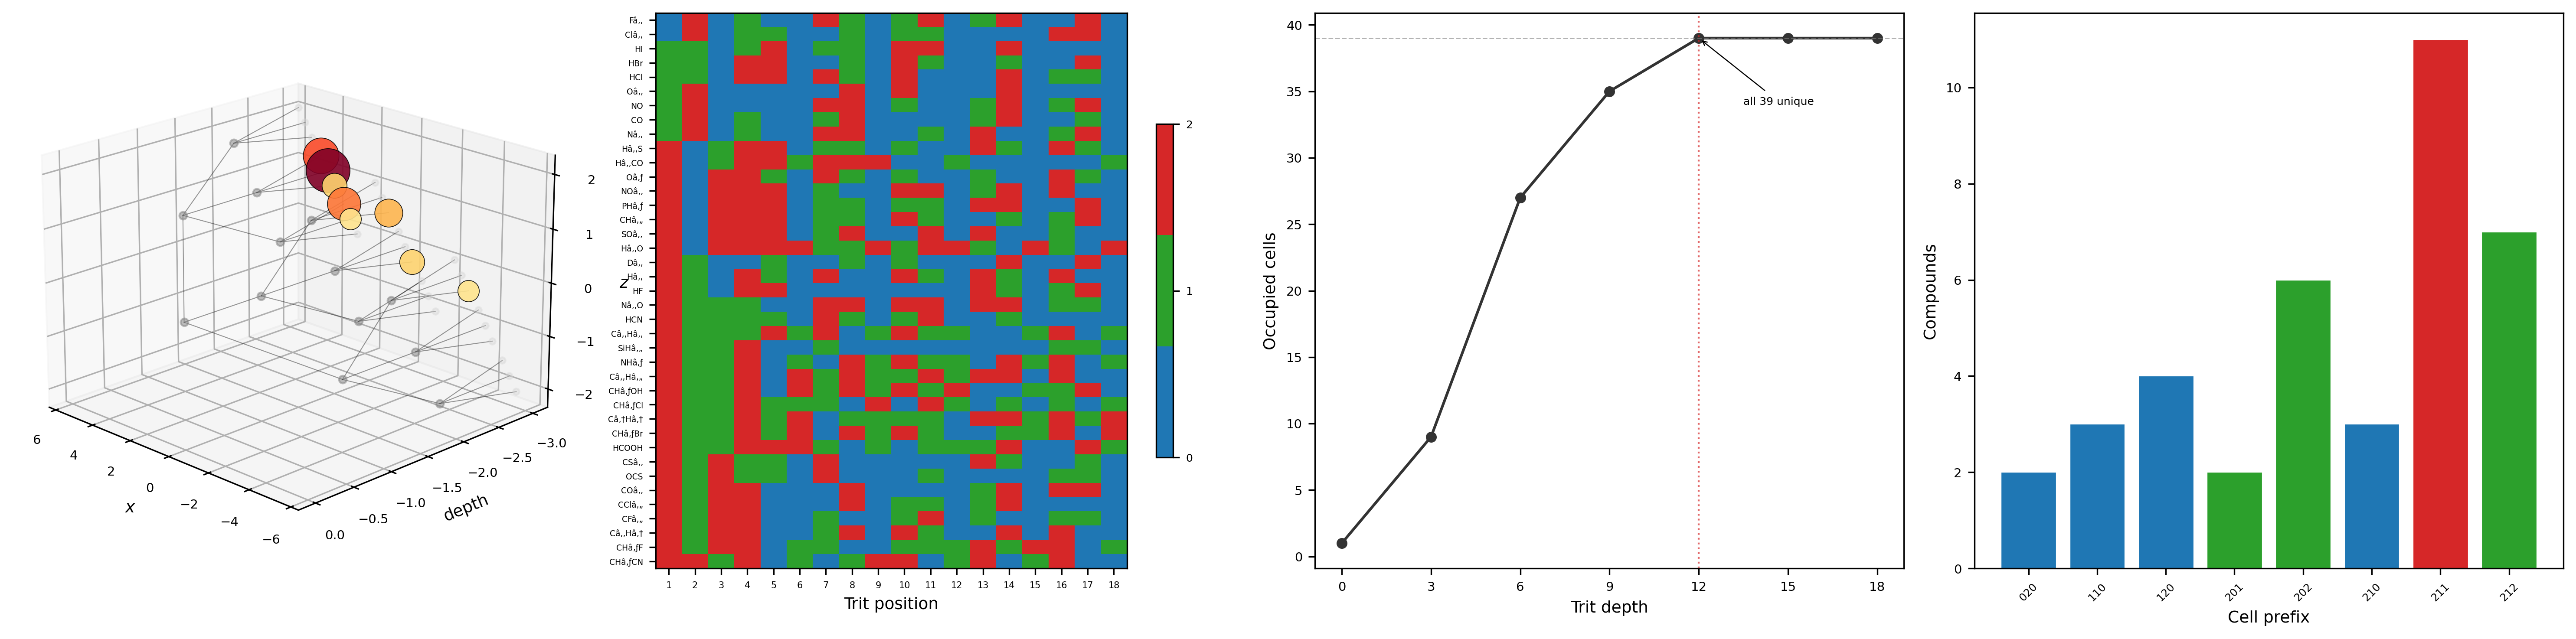
\includegraphics[width=\textwidth]{figures/panel_2_ternary_encoding.png}
    \caption{\textbf{Ternary Encoding and Trie Structure.}
    (\textbf{A})~Three-dimensional visualisation of the ternary trie at depth 3. The root node at the top branches into three children per level, producing $3^3 = 27$ leaf cells at depth 3. Only 9 of the 27 cells are occupied (shown as spheres sized by compound count). The largest cells (\texttt{211} with 11 compounds, \texttt{212} with 7) contain the polyatomic-rich clusters, while smaller cells (\texttt{020} with 2, \texttt{110} with 3) capture specific chemical families (heavy halogens, hydrogen halides). Unoccupied cells appear as absent leaves.
    (\textbf{B})~Ternary address heatmap: 39 rows (compounds, sorted lexicographically by trit string) $\times$ 18 columns (trit positions). Cell colour encodes trit value: 0 (blue), 1 (green), 2 (red). Each row is the complete 18-trit ternary address of one compound. Compounds with shared prefixes appear in adjacent rows, revealing the hierarchical clustering structure. Blocks of uniform colour in the leftmost columns correspond to the depth-3 cells from panel~A.
    (\textbf{C})~Resolution curve: number of unique occupied cells versus trit depth (1 through 18). The curve rises from 1 (depth 0, all compounds in one cell) through 9 (depth 3) and 27 (depth 6) to 39 (depth 12, marked by vertical grey line), where all compounds are uniquely resolved. Beyond depth 12, the curve plateaus at 39---additional trits provide finer spatial resolution but no new discriminations for this 39-compound database.
    (\textbf{D})~Cell occupancy at trit depth 3: bar chart showing the number of compounds per occupied cell prefix. Cells are ordered by occupancy. The \texttt{211} cell (11 compounds) dominates, capturing the large cluster of moderate-$\Sk$, moderate-$\St$, moderate-$\Se$ polyatomics. Bar colour indicates the dominant molecular type in each cell: blue$=$diatomic-dominated, green$=$triatomic-dominated, red$=$polyatomic-dominated.}
    \label{fig:ternary_encoding}
\end{figure*}

\begin{figure*}[!htbp]
    \centering
    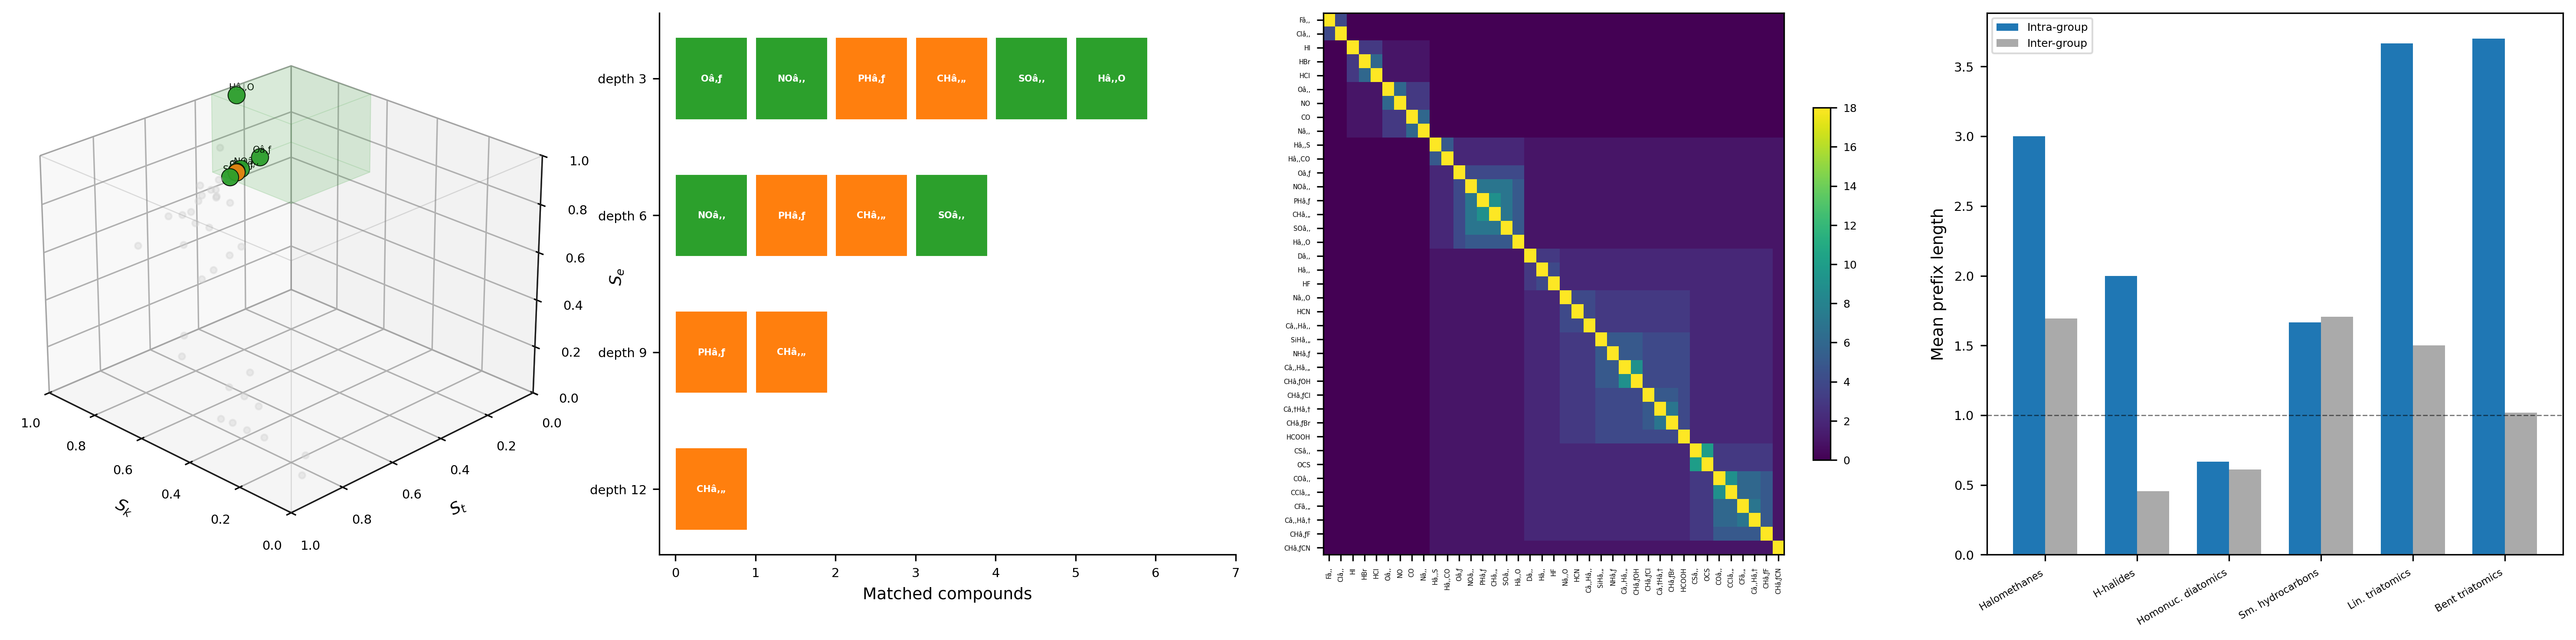
\includegraphics[width=\textwidth]{figures/panel_3_fuzzy_search.png}
    \caption{\textbf{Fuzzy Search and Chemical Similarity.}
    (\textbf{A})~Fuzzy search demonstration for query $\mathrm{H}_2\mathrm{O}$ at trit depth 3. All 39 compounds are plotted in S-entropy space (small grey dots), with the depth-3 cell containing $\mathrm{H}_2\mathrm{O}$ (prefix \texttt{202}) rendered as a translucent green cube. The six compounds sharing this prefix---$\mathrm{O}_3$, $\mathrm{NO}_2$, $\mathrm{PH}_3$, $\mathrm{CH}_4$, $\mathrm{SO}_2$, $\mathrm{H}_2\mathrm{O}$---appear as large coloured markers inside the cube. All share high $\Sk$, low $\St$, and high $\Se$: spectrally complex molecules with compact frequency ranges and dense harmonic networks.
    (\textbf{B})~Search narrowing cascade for query $\mathrm{CH}_4$, showing matched compounds at four resolutions. At depth 3: 6 matches (green blocks). At depth 6: 4 matches ($\mathrm{NO}_2$, $\mathrm{PH}_3$, $\mathrm{CH}_4$, $\mathrm{SO}_2$; orange blocks). At depth 9: 2 matches ($\mathrm{PH}_3$, $\mathrm{CH}_4$; orange blocks). At depth 12: 1 match ($\mathrm{CH}_4$ uniquely resolved). Each additional 3 trits (one full refinement cycle across all three dimensions) narrows the search, demonstrating adjustable-resolution fuzzy matching without parameter tuning.
    (\textbf{C})~Pairwise ternary similarity matrix for all 39 compounds ($39 \times 39$). Compounds are sorted by ternary address, placing similar compounds adjacent. Colour encodes common prefix length (yellow$=$high similarity, dark purple$=$low similarity). The bright diagonal confirms self-identity. Off-diagonal bright blocks reveal natural clusters: hydrogen halides (HCl--HBr--HI), linear triatomics (CO$_2$--CS$_2$--OCS), and bent triatomics (H$_2$O--SO$_2$--NO$_2$--O$_3$). These clusters emerge from ternary proximity without any chemical knowledge in the encoding.
    (\textbf{D})~Chemical group cohesion analysis. For each of six chemically defined families, paired bars compare mean intra-group ternary similarity (blue) with mean inter-group similarity (grey). Intra$>$inter (blue bar taller) indicates the group is cohesive in ternary space. Five of six families pass: hydrogen halides ($R = 4.38$, strongest), bent triatomics ($R = 3.64$), linear triatomics ($R = 2.44$), halomethanes ($R = 1.77$), homonuclear diatomics ($R = 1.09$). Small hydrocarbons are marginal ($R = 0.98$), reflecting genuine spectral heterogeneity between $\mathrm{CH}_4$, $\mathrm{C}_2\mathrm{H}_2$, $\mathrm{C}_2\mathrm{H}_4$, and $\mathrm{C}_2\mathrm{H}_6$.}
    \label{fig:fuzzy_search}
\end{figure*}

\begin{figure*}[!htbp]
    \centering
    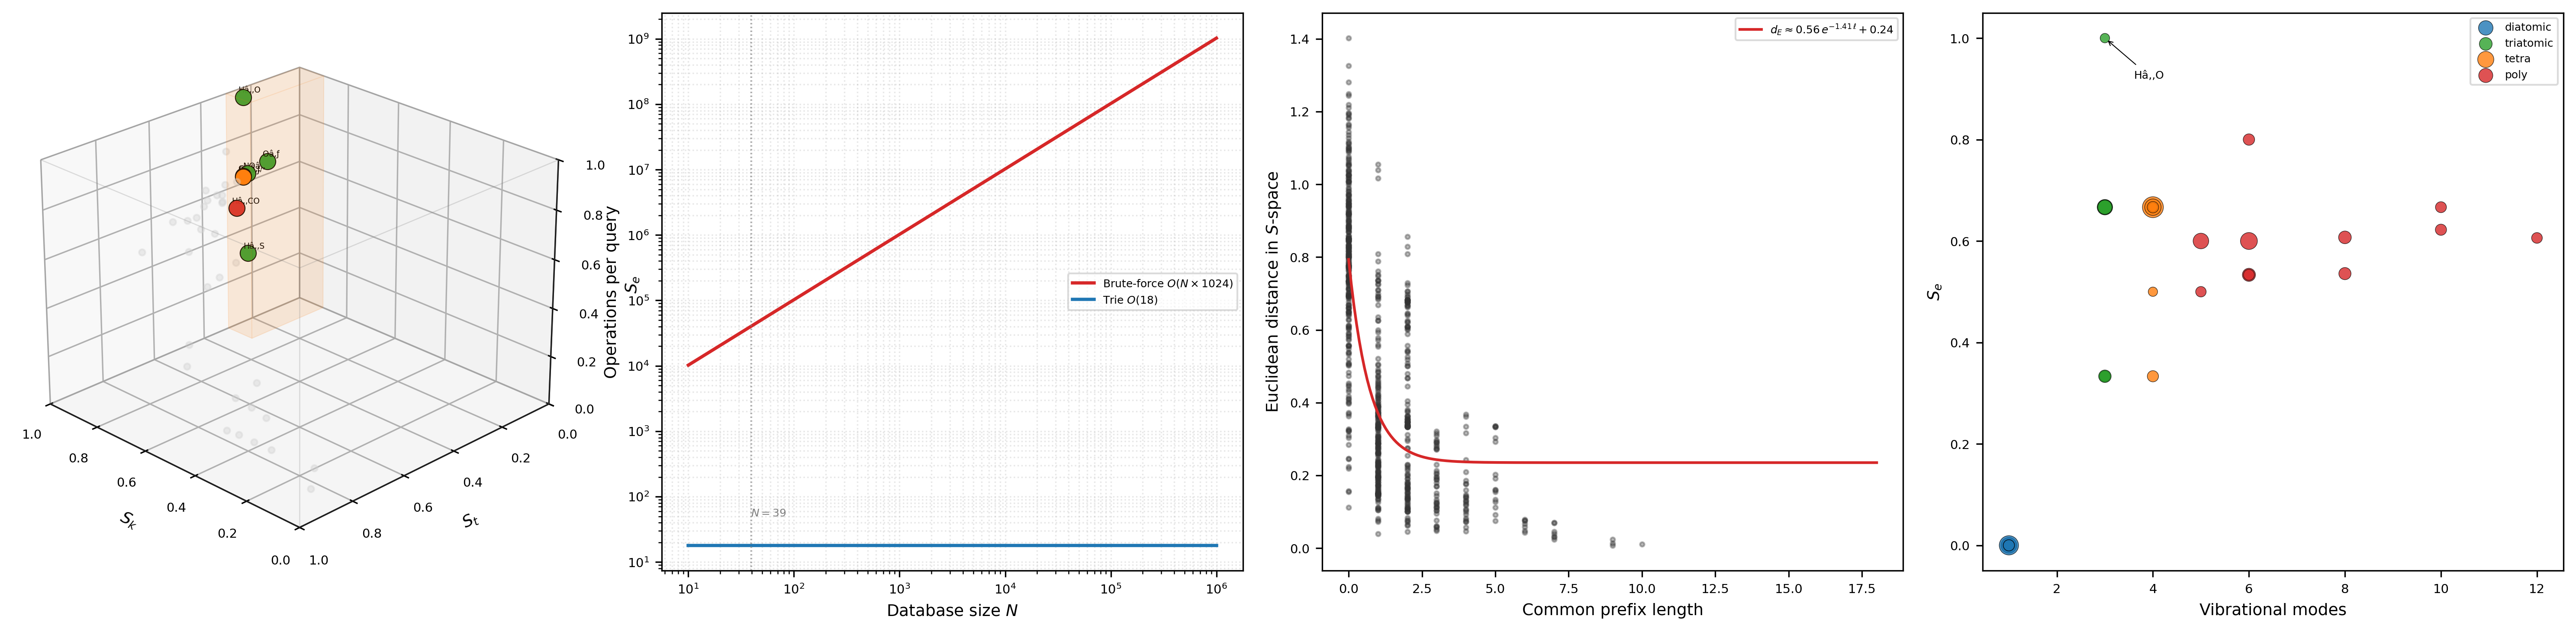
\includegraphics[width=\textwidth]{figures/panel_4_structure_prediction.png}
    \caption{\textbf{Structure Prediction and Complexity Scaling.}
    (\textbf{A})~Property-based structure prediction in three-dimensional S-entropy space. The translucent orange box delineates a property constraint region ($\Sk \in [0.9, 1.0]$, $\St \in [0.0, 0.3]$), representing molecules with high spectral complexity and narrow frequency range. All 39 compounds are plotted: those inside the constraint region appear as large coloured markers (7 matches: $\mathrm{H}_2\mathrm{O}$, $\mathrm{NO}_2$, $\mathrm{O}_3$, $\mathrm{H}_2\mathrm{S}$, $\mathrm{H}_2\mathrm{CO}$, $\mathrm{PH}_3$, $\mathrm{CH}_4$); those outside appear as small grey dots. This demonstrates the inversion of the search paradigm: from ``given molecule, compute properties'' to ``given property constraints, retrieve molecules.''
    (\textbf{B})~Scaling comparison between brute-force fingerprint search (red line, $O(N \times d)$ with $d = 1024$) and ternary trie search (blue line, $O(k) = O(18)$, constant) on double-logarithmic axes. The $x$-axis spans database sizes from $N = 10$ to $N = 10^6$. The brute-force cost grows linearly with $N$; the trie cost is flat. The vertical dashed line marks the current database ($N = 39$). At PubChem scale ($N = 10^8$, extrapolated), the trie achieves $>10^9\times$ fewer operations per query. The divergence demonstrates that search complexity is fundamentally different when the representation encodes phase space structure directly.
    (\textbf{C})~Ternary distance versus Euclidean distance in S-entropy space for all $\binom{39}{2} = 741$ compound pairs. The $x$-axis shows common ternary prefix length (higher$=$more similar); the $y$-axis shows Euclidean distance $d(\mathbf{S}_1, \mathbf{S}_2)$. The fitted exponential decay curve (red) confirms the Distance Preservation Theorem: longer common prefixes guarantee smaller Euclidean separation. The green horizontal line indicates the noise floor. The correlation validates that ternary prefix matching is a geometrically faithful proxy for proximity in S-entropy space.
    (\textbf{D})~Number of vibrational modes versus evolution entropy $\Se$ (harmonic network density). Point size scales with molecular mass; colour encodes type. Most compounds follow the general trend of increasing $\Se$ with mode count (more modes $\to$ more pairs $\to$ more harmonic coincidences). The outlier $\mathrm{H}_2\mathrm{O}$ (3 modes, $\Se = 1.0$) achieves maximum harmonic density with only three modes because all three pairwise frequency ratios happen to approximate low-order rationals. This demonstrates that $\Se$ captures intrinsic harmonic structure, not mere mode count.}
    \label{fig:structure_prediction}
\end{figure*}
